\newcommand{\waInputStyles}{\texttt{se-wa-input-styles-v097.tex}}

\chapter{Anhang}

\begin{figure}[H]
\centering
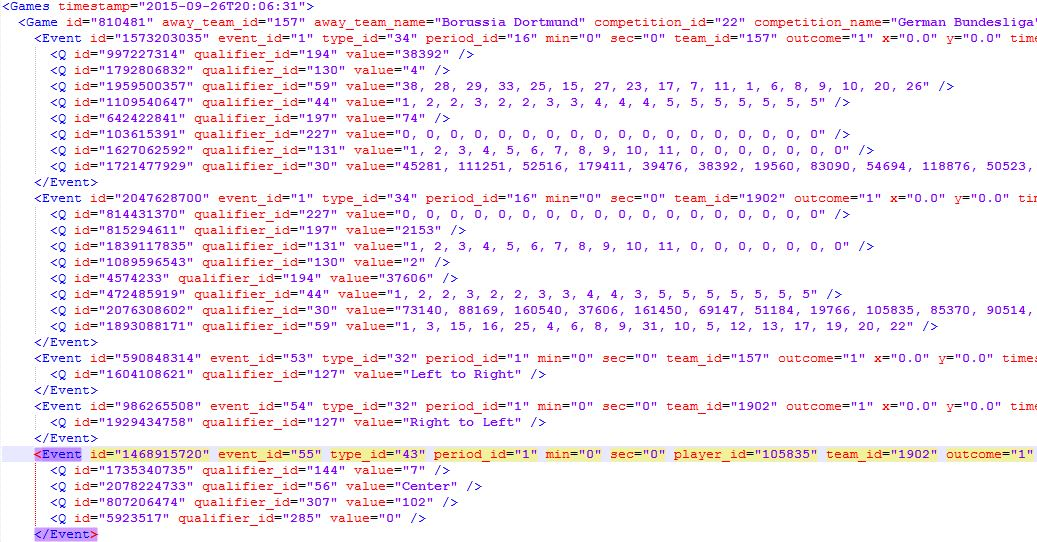
\includegraphics[scale=0.52]{se-wa-jpg/daten}
\caption{Auszug aus der XML-Datei mit den Events}
\label{xmldaten}
\end{figure}

Die \vref{xmldaten} zeigt einen Ausschnitt aus der XML-Datei in der alle Events eines Spiels aufzeichnet sind. Im oberen Teil sind die Mannschaftsaufstellungen zu sehen, wobei jeder Spieler eine eigene ID besitzt. Darunter folgt gelb markiert zum Anpfiff der Partie der erste Pass mit dem \textit{Outcome} 1, welcher einen erfolgreichen Pass identifiziert. 

\chapter{MatLab Code}